%Calculate the cognitive salience index (sutrop 2001) and compare to values of difficulty of single words from the model

%Mention friends network and peer to peer transmission of knowledge!!!

%%%%%%%%%%%%%%%%%%%%%%%%%%%%%%%%%%%%%%%%%%%%%%%%%%%%%%%%%%%%%%%%%%%%%%%%%%%%%%%%%%%%%%%%%%%%%%%%%%%%%%%%%%%%%%%%%%%%%
%%%%%%%%%%%%%%BIN%%%%%%%%%%%%%%%%%%%%%%%%%%%%%%

We hope to correlate certain aspects of life history to knowledge variation, and to explain part of this variation with additional aspects of children and teenager behaviors.


% lit review sex differences
Another pattern that often emerged in studies estimating knowledge in boys and girls, is a difference between the sexes (\cite{Blacutt-Rivero2016LocalBolivia}). But when content was included in the analysis, it appeared that boys and girls often focused on different aspects of ecological knowledge. 
%CHECK THIS PARAGRAPH FOR CORRECT CONTENT
These differences are not expected to be innate, but rather are linked to the differential engagement in sex specific activities related to different subsets of our ecological niche. 
Detailed analyses of gender specific areas of knowledge is missing. Most studies either focus on one aspect of ecological knowledge, often gender specific ones such as fishing (\cite{Koster2016WisdomElders}), or do not explore the variation between sexes in terms of content. 

%what sex diff tell us
Exploring gender differences can inform the discussion on the importance of knowledge for life history in multiple ways. First, the timing of emergence of gender differences in knowledge could be correlated to that of other differences between gender, such as labor division or sexual maturation.
Second, the fact that certain activities are associated to one of the sexes generates enough variation to quantify the effect of activities practiced, which would be important to make inferences on the importance of practice for the acquisition of knowledge.
Third, exploring how the two genders differ in the aspects of ecological knowledge on which they can clarify what is the importance of learning about the environment in relation to its economical function. 
%review this sentence


%Finally, our analysis attempts at disentangling the effect on total knowledge of different components.

%Humans are weird. We need knowledge
%It is not hot news that our species exhibit several traits, that, taken together, arrange themselves in a peculiar constellation.For a start, we live in every kind of environments on almost every continent. We exploit diverse ecological niches, relying on a wide variety of food sources, which are irregularly distributed in time and space. A large proportion of our diet is composed of hard-to-get resources with high nutrition value, that we we are not physically adapted to obtain. We instead use vasts arrays of technologies to access these resources, technologies that could never be invented in a single lifetime. We coordinate with many other individuals in our attempts to guarantee our livelihoods and follow complex social norms when interacting. All of these aspects of our foraging strategies require vast amount of knowledge. And, be it through individual or social learning, we need time to acquire this knowledge. 

%Lack of terminology consensus within and across disciplines complicates the discussion that follows(\cite{meehan2016childhood}), but I will treat here infancy the period of exclusive dependency of young humans, that ends roughly with weaning around 3-4 years of age, childhood as the period between infancy and adolescence, when somatic growth decelerates, the brain reaches full size and individuals start to be at least partially producers, and adolescence, when a growth spurt brings the body to adult height and sexual traits reach maturation. 
%Childhood is a human-specific phase of early life history that inserts itself between infancy and the juvenile period, rougly between 3 and 12 years of age. It is characterized by a reduction in the speed of somatic growth, whereas it is in tis period that the brain reaches its adult size. 

%the emergence of childhood, a period of human lives when xxxx happens, The pattern of growth typical of our juveniles, with the slow down of physical growth between xxx and xxx years of age,could be an adaptation to allow our brains, reaching by now adult size, to be filled with large amounts of the required information. 

%but we don't understand behavioral changes
%Our understanding of behavioral changes during childhood and adolescence is more limited than that of somatic changes. 
%Developmental psychology tackles the issue with different goals.
%Observational studies of behavioral changes tell us something about emergence of labor division and learning strategies.
%Acquisition of knowledge in time
%labor division, activities
%knowledge
%Some studies tried to measure the increase of knowledge with age in a variety of mixed subsistence societies. 
%Knowledge increases with age, there are gender differences in amount of knowledge. 

%what are we going to do
%We focus on ecological knowledge for a variety of reasons, but especially because an understanding of the environment is expected to have actual consequence on the livelihood of individuals who rely at least partially on foraged foods or small scale agriculture. Also, local ecological knowledge, or LEK, is an easily sub-settable portion of knowledge to explore and is considered important in the preservation of traditional cultures as well as wildlife.  

%A better understanding of the other factors influencing knowledge would also be helpful. Especially, most studies find a difference in knowledge between sexes, in total knowledge or in knowledge by area. Boys are more experienced when talking about animals and girls about plants %FIIIIIIND?!?!?
%This division would be associated to sex division of labor, hunting being a typical male activity, whereas gathering of plants is more commonly a female one. Understanding the emergence of differences in knowledge of the natural environment would be cool.

%in the supplementary we also show the effect of other things
%Finally, mixed evidences on the effect of formal schooling, presence of specific members of the family or sibship order have been investigated as factors influencing individual knowledge, so we look at these here as well.

%In order to contribute to the discussion on the importance of knowledge, we collected data in a population of partial time foragers and analyzed them with a set of Bayesian latent models. 

%HINT AT MULTIPLE DIMENSIONS OF KNOWLEDGE

%The income generated by the clove market brings a relief in the mostly cashless economy of the village, although is not reliable and in any case it is limited to the clove harvesting season. Alternative sources of money are the cultivation of algae for the Asian market, which is labor intensive and pays really badly, and production of charcoal. 

\begin{figure}[h]
    \begin{tikzpicture}
        \node (AGE) [rec] {Age};
        \node (SEX) [rec, left=0.8 of AGE] {Sex};
        \node (FAM) [rec, right=0.8 of AGE] {Family};
        \node (ACT) [rec, below=1 of SEX] {Activities};
        \node (SCH) [rec, below=1 of FAM] {Schooling};
        \node (K) [rec, below=3 of AGE] {Knowledge};
        \draw[->,line width=0.7] (AGE) -- (K);
        \draw[->,line width=0.7] (AGE) -- (ACT);
        \draw[->,line width=0.7] (AGE) -- (SCH);
        \draw[->,line width=0.7] (SEX) -- (ACT);
        \draw[->,line width=0.7] (SEX) -- (SCH);
        \draw[->,line width=0.7] (FAM) -- (ACT);
        \draw[->,line width=0.7] (FAM) -- (K);
        \draw[->,line width=0.7] (FAM) -- (SCH);
        \draw[->,line width=0.7] (ACT) -- (K);
        \draw[->,line width=0.7] (SCH) -- (ACT);
        \draw[->,line width=0.7] (SCH) -- (K);
    \end{tikzpicture}
    \caption{DAG describing relation between analyzed variables.}
    \label{fig:DAG}
\end{figure}



\begin{figure}[h]
    \begin{tikzpicture}
        \node (HID) [rec] {Household};
        \node (SSP) [rec, right=1 of HID] {Same sex parent};
        \node (SEX) [rec, right=1 of SSP] {Sex};
        \node (PPP) [rec, below=1 of SSP] {Presence of parents};
        \node (ACT) [rec, below=1 of SEX] {Activities};
        \node (FBO) [rec, below=1 of HID] {Firstborn};
        \node (BOR) [rec, below=1 of FBO] {Birth order};
        \node (K) [rec, below=1 of PPP] {Knowledge};
        \draw[->,line width=0.7] (HID) -- (K);
        \draw[->,line width=0.7] (HID) -- (PPP);
        \draw[->,line width=0.7] (HID) -- (SSP);
        \draw[->,line width=0.7] (PPP) -- (K);
        \draw[->,line width=0.7] (SSP) -- (PPP);
        \draw[->,line width=0.7] (SEX) -- (SSP);
        \draw[->,line width=0.7] (SEX) -- (ACT);
        \draw[->,line width=0.7] (BOR) -- (K);
        \draw[->,line width=0.7] (FBO) -- (BOR);
        \draw[->,line width=0.7] (ACT) -- (K);
    \end{tikzpicture}
    \caption{DAG describing relation between analyzed variables.}
    \label{fig:DAG}
\end{figure}

%model
%Data were analyzed using a Bayesian IRT model developed in Stan. IRT models, initially developed as a mean to grade tests in pedagogy, aim at estimating one or multiple latent traits, such as knowledge, from answers to questions. They estimate individual level traits while simultaneously allowing questions to vary in difficulty ($\beta$) and discrimination($\alpha$). The model treats the three different types of questions independently, estimating simultaneously the two main parameters for the freelist and image recognition tests (2PL) and also probability of guessing for the questionnaire (3PL), which include probability of guessing ($\gamma$), while estimating also a knowledge parameter for each interviewee ($K$). Knowledge is intended as a latent trait influencing the probability of naming a certain object in the freelist, of answering correctly to the questionnaire or of listing each of the creatures appearing in the images.

%$K$ in turn is estimated with a generalized linear model that estimates the effect of individual level traits on knowledge. These include: Age ($A$) (as reported by the children themselves), sex ($S$), activities performed ($AC$), time spent in school ($SY$) and several family related factors. An individual intercept absorb remaining variation. 
%Multiple models have been constructed to infer the relevance of the factors just described 
%if other things are included in the definition of age, add here
%time spent in school ($SY$), estimated using as a proxy the grade in which students are currently enrolled or that they have completed last, assuming that older children enrolled in earlier classes have spent less time in school or school related tasks;

\begin{figure}
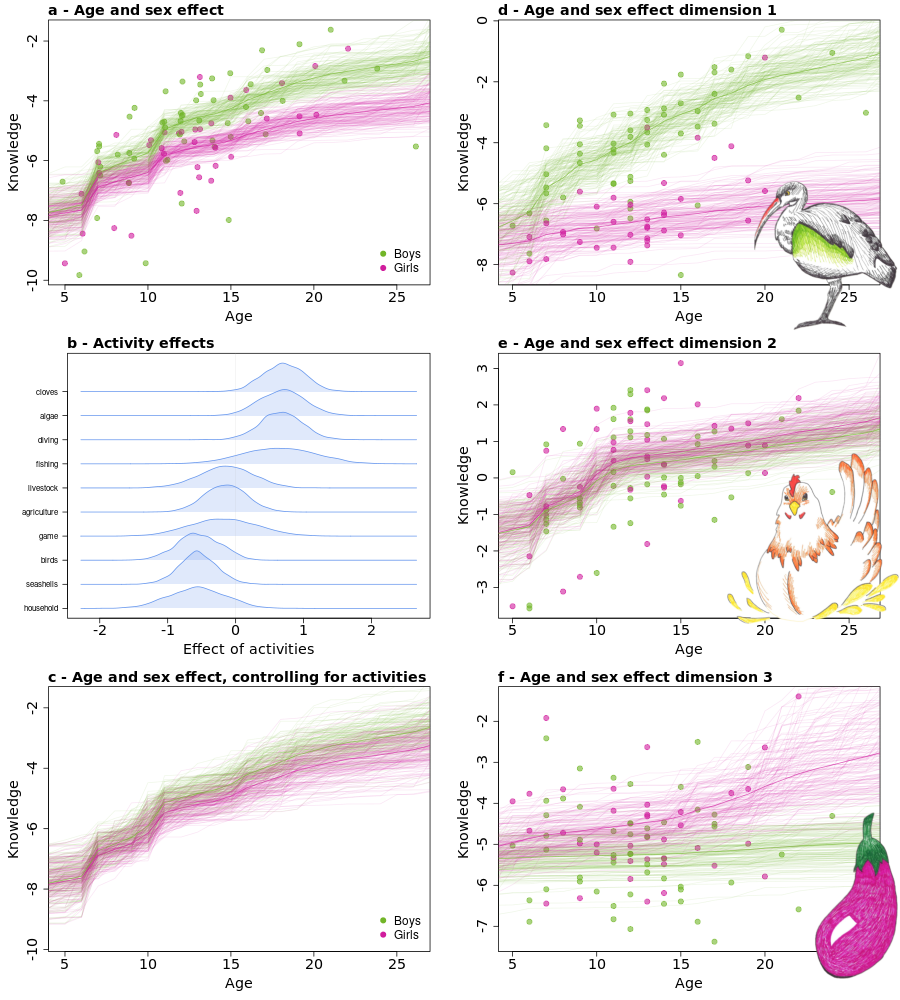
\includegraphics[width=12cm]{4_Outputs/plots/exaptychpics.png}
\caption{\textbf{Graph a} shows knowledge of individuals $K_i$ estimated from Model 1 for individuals over their age, color coded for sex. The curves represent estimated knowledge at each age per sex, each line a set of values from the posterior sample. $K_i$ values are mean of the posterior distribution for the relative values. \textbf{Graph b} shows mean and 89\% confidence intervals CI for the activity parameters $bAC_actvity$. \textbf{Graph c} shows increases of knowledge for age and sex in a counterfactual condition in which individuals practice no activity. \textbf{Graphs d-f} show individual knowledge $K_i,d$ estimated in each of three different dimensions, color coded for sex. The cartoons represent one of the most salient species in each dimension.}
\label{fig:quadriptych}
\end{figure}




%These older kids, however, show a very good knowledge of the environment. These individuals routinely listed more than 100 plants and animals, with the more knowledgeable going over 200. 



The analysis of dimensions further helps us explain sex differences and age related effects. From the WAIC results, it appears that including a higher number of dimensions helps predicting out of sample accuracy (see supplementary). After 3 dimensions, though, the increases in accuracy are minimal, suggesting that 3 dimensions are enough to describe the data appropriately. Figure \ref{fig:quadriptych}, graphs d to f, shows estimated knowledge for individuals in each of the three dimensions, plus dimension -and sex- specific increases with age. Each dimension picks up a specific trend from the data. In one of the dimensions, boys and girls learn at the same rate and achieve a similar total knowledge. Of the remaining two dimensions, one shows significant increase in knowledge for boys, and the other for girls, whereas the opposite sex seems not to learn at all. The trends of increases with age differ in the three dimensions. Dimension 1 sees the boys pick up knowledge at high speed, and does not show strong signs of leveling off in later ages. Girls learn much more slowly in this dimension, if at all.  In the second dimension, boys and girls do not differ in the amount of knowledge per age, and have similar age trends. Specifically, knowledge increases significantly until when individuals are about 12 years old. After that, knowledge plateaus. Dimension 3 is the least descriptive of the data, and the trends are less certain. It appears, though, that girls' knowledge in this dimension increases during adolescence, while boys do not learn at all. The most salient items in this dimension are  

Now let’s look at the difference between genders. 

In figure \ref{fig:activities_years}, we can see how m
We then proceeded to analyze the same model, but including the effect of practicing a certain activity. Looking at the parameters $bAC$, describing the effect of each activity on knowledge, we can see that there's a certain amount of variation (Figure \ref{fig:quadriptych}, graph b). Some activities have almost no effect, some others, such as hunting birds, have a positive effect on knowledge, and finally activities such as household chores, have a negative effect (see supplementary for distribution parameters of the posterior). 

When including activities as a covariate, the difference in knowledge between the sexes decreases significantly. We can see this from how much the lines for male specific and female specific knowledge overlap, in Figure \ref{fig:quadriptych}, graph c. But when controlling for activities, the difference between the sexes reduces, and the posterior distributions for the sex specific age effects $bA_s$ overlap. This means that activities explain at least part of the variation in knowledge between the sexes. 

%curve slowing down with age because it follows the fact that there is less to learn. If individuals keep learning the same proportion of what is left to learn each year, they learn a lot when they're young and less when they're older. So knowledge doubles from when you're 10 to 20, but it doesn't keep going that way later on. Still learning but less.
%compare with chimps - by 10 they're fully developed and autonomous
 But this is simply a mechanistic view, and the rates of knowledge acquisition over age reveals other interesting patterns. 



%\cite{Quinlan2016ChildrensVillage} Cross-culturally, LEKincreases substantially between the ages of nine and 12,  reaching adult levels sometime duringadolescence (Hewlett and Cavalli-Sforza 1986; Luczaj and Nieroda 2011; Stross 1970; Zarger 2002;Zarger and Stepp 2004).  Many children in subsistence societies are masters of their natural envi-ronment by the age of 12 (Hewlett and Cavalli-Sforza 1986; Hunn 2008; Stross 1973)/// they have a plant trail, which is good but limits possible knowledge to a maximum of plants recognizable (strong ceiling effect), thus loosing specialized knowledge in certain areas, which is potentially very large. (acquiring specialized knowledge can happen later in life, while most of the general knowledge might be learned earlier)



%\cite{Bortolotto2015KnowledgeBrazil} says that knowledge is the highest among older people (>60)


%By the time kids are 10, their brain have reached more or less their full size, but they’re not done filling up with information. They will learn about as much as they have already learnt by the time they’re 20, and will most likely keep learning, although much less. 

%Boys appear to know a little bit more about the natural environment than girls do. This was not a surprise to us, as gender differences have been observed before.
%, just when labor division starts to emerge. As we do not believe there’s some innate difference between sexes in knowledge, but on the contrary we think this emerges from sex specific engagement with activities, this was a first interesting result. 

%Describe activities by types (requiring knowledge- not requiring knowledge) and notice details: Seashell collection, which is also mostly practiced by girls, has a positive effect, and it’s an activity which probably promotes the knowledge of some specific areas. Spearfishing and hunting with dogs might not increase knowledge after childhood, and just strength is required. 

%sex differences in knowledge are not innate, they emerge as individuals go on and practice different activities

%activities are obv not the only thing that contributes to increases in knowledge with age, although once controlled for activities the total effect of age is reduced. Knowledge, though, increases with age even controlling for activities, suggesting that even hanging around people provides means to increase ecological knowledge.

%dimensions - first time ecological knowledge is analyzed with dimensions, can better look at where are differences between the sexes
%simple items talk about not really knowledge, but areas of interest
%Discuss content of dimensions and age specific patterns per dimension - with general knowledge for early ages and specialization in adolescence.

%they're also trading off learning for the future with current returns, and the whole system is in a complex equilibrium - somatic growth slows down until when they can actually contribute substantially to their own maintenance (although for sure a certain portion of foraged resources can be acquired only with a larger soma - so hard to tell).


The fact that the largest increase in knowledge happen between 7 and 12 years (Figure \ref{fig:quadriptych}-a) calls our attention to the juvenile period, when children start to engage more with the world around them. Just as the brain reaches adult size, it gets filled with information, while children become more independent and perform productive activities with some regularity, if with different level of success. The knowledge they acquire during this phase seems to be very generic, as if children were tapping into the easier, most common part of all the available knowledge. They learn about their environment, and start to use it in real world activities, but this is not enough to render them autonomous. By this time, children often have one or more younger siblings and are not the main concern of their parents anymore. They usually produce a consistent proportion of their caloric needs, which are kept low by a prolonged period of slow somatic growth,  but are still dependent from adults for protection and provisioning. the brain reaches adult size, it gets filled with information, while children become more independent and perform productive activities with some regularity, if with different level of success children often have one or more younger siblings and are not the main concern of their parents anymore. They usually produce a consistent proportion of their caloric needs, which are kept low by a prolonged period of slow somatic growth.In particular, they are usually not skilled enough to perform many adult activities, but rather focus on a subset of children-specific tasks. 
During this time, the difference in total amount of knowledge between the sexes is barely perceptible, and most of the information acquired is shared between sexes.

Following this period, adolescence is a time in which knowledge acquisition continues at a slower rate. Sex specific knowledge accounts for most of the increases in this phase of life, with boys learning male-specific information at a constant rate, and girls doing some gendered learning. The dimension of knowledge in which males keep improving all through adolescence and later on seems to be focusing on bird and fish species. Males in this population do all the hunting and fishing, and keep acquiring knowledge linked to these activities all through their lives -at least in the sampled period. They start learning very early, having a higher knowledge in this dimension already during early childhood, but the distance increases with time, and accounts for most of the difference in total knowledge between sexes. Girls seem to have a sex specific dimension of knowledge, linked to edible vegetables and seashells and maybe medicinal plants, but the limited data from older girls and young women makes it hard to make strong claims in this direction. General knowledge does keep increasing during adolescence, but at a much slower rate, almost imperceptibly so. 
The fact that gender plays such a big role in knowledge acquisition during adolescence is probably linked to the fact that by this time individuals fit in distinguished gender roles, with clear division of labor and sex specific activities. 

The importance of dimension of knowledge activities themselves is reinforced by fact that gender differences in total knowledge almost disappear when they are taken into account (Figure \ref{fig:quadriptych}-c). The difference in knowledge between boys and girls seem to be mostly driven by certain sex specific activities, such as bird hunting and fishing (Figure \ref{fig:quadriptych}-b), which are mainly practiced by males and promote the acquisition of male specific knowledge in Figure \ref{fig:quadriptych}-d. Interestingly, activities such as seashell collection, which is the only female oriented activity that involves interacting with the natural environment, also has a positive effect on knowledge acquisition. On the contrary, household chores have a negative effect (Figure \ref{fig:quadriptych}-b). This reinforces the idea that certain activities are important for the acquisition of knowledge, and the time invested in practicing these activities results in knowledge that is specific to that activity. 

The total amount of knowledge seems to plateau after 20 years of age, suggesting that most of the knowledge acquisition has taken place by this point. Our data does not include a sufficient number of young adults to support strong inferences on the later stages of life, but it appears that, after adolescence, any increase in knowledge would be in sex specific domains. It is possible that certain individuals will keep learning about the natural environment as they might become local expert in medicinal plants or fishing, but most individuals have reached a good amount of knowledge by this time. Older individuals in \cite{Koster2016WisdomElders} are considered very knowledgeable, but, once measured, their knowledge does not actually differ much from that of younger adults. This pattern could be due to some sort of ceiling effect, for example if individuals reach a maximum number of species listed in a freelist for memory limitations, but it also could simply be due to the fact that old people are considered experts in many subjects just due to their age. 



 dimension of knowledge activities
%disproving hawkes idea of general elongation - there seem to be a role of learning in evolution of childhood - at least knowledge increases + what we do and whom we stay with are important for learning, so time is not all the same, it has a purpose

%trade off current learning vs future returns
%distinguish between knowledge, applied knowledge and skill (e.g. ppl can climb trees and collect stuff, and name the plant, but can't find it in the wild cause that's another knowledge)
(this mainly involves moving one or more tethered cows from one patch of grass to the other and bringing them to drink to the river)

, the shape of their knowledge over age wouldn't be too different from what we observe in figure \ref{fig:age-sex}, some sort of decelerating function.
But this function can flex and level off earlier or later.
Chimpanzees, for example, appear to have learned most of what they need to know by 10 years of age, or at least, by that age, their foraging behavior does not differ from that of an adult \citep{BrayTheSchweinfurthii, Lonsdorf2021WildWeaning}. Children could be slower learners, or they might have a higher mountain to climb, in terms of knowledge to acquire. Just by looking at some raw numbers from our results, we would be lured to lean toward the second hypothesis: 

And this is only one aspect of our social and productive life.  
Weakly informative normal priors centered on 0 were used for the varying effects ($\alpha$ and $\eta$), for activity specific fixed effects ($\gamma$) and for fixed effects of co-residence with parents ($\psi$, $\phi$). Scale parameters ($\sigma_{\alpha}$ and $\sigma_{\eta}$) were assigned exponential priors. Sex specific age effect $\beta$ had a truncated normal prior. Year specific incremental effects of age $\delta$ had a weak Dirichlet prior ($\alpha = 0.5$). 
For question parameters $a$, $b$ and $c$ we used, respectively, positive truncated normal (mean = 0, sd = 1), normal (mean = 0, sd = 2) and beta distributions ( $\alpha = 5$ and $\beta = 10$, which is a continuous distribution in the interval [0,1]).


Finally, the results relative to the dimension analysis improve our understanding of the complexity of ecological knowledge, by highlighting the presence of multiple distinguishable, gender specific areas of it. The fact that no other study performed a similar kind of analysis leaves this single result to be an inadequate representation of human knowledge. Cross cultural comparisons and contextualized analyses are needed to support any generalizable conclusion on knowledge dimensionality or differences among the sexes, but our observation opens the path for a clearer approach to studying knowledge of the environment. Contrasting results from previous studies on gender differences in local ecological knowledge could be coherent with our interpretation of dimensions. Indeed, studies using data from a freelist task, such as \cite{Cruz-garciaChildrenThe}  and \cite{Geng2016TraditionalProvince}, found no difference comparing the total number of items listed. On the contrary, when delving into the details of their knowledge of palm uses, \cite{Blacutt-Rivero2016LocalBolivia} found that boys and girls do not share the same knowledge and, more extensively, \cite{Schniter2021Age-AppropriateChoyeros} find substantial differences in the knowledge adult men and women have of different areas of the environment. These are cases in which the approach to data collection, as well as the analysis, can impact the outcome of a study. Techniques such as freelisting allow subjects to explore all possible areas of knowledge, and for example women and men can list a similar total number of items, but different species. On the contrary, data collection procedures which require more agency of the researchers can be biased by their previous expectations or knowledge and fail to represent all areas of knowledge (see SI \ref{SI:data_details} for some more thoughts on how this issue influenced the present study).



%Gender is important because of the prevalence of a sexual division of labour in most productive activities involving the natural environment (Bird 1999) . Gendered differences in knowledge are often (REFS? Blacutt-Rivero et al., 2016, Cruz-garcia et al., Geng et al., 2016, Schniter et al., 2021]) but not always (REFS, Blacutt-Rivero et al., 2016, Cruz-garcia et al., Geng et al., 2016, Schniter et al., 2021]) observed, and our specific contribution in this area is to show how gendered differences in knowledge are related to the differential engagement in sex specific activities in different subsets of the ecological niche), thereby more explicitly downplaying inferences regarding innate contributions. 


% lit review on what has been done
%Past research has focused on ecological knowledge because of its importance for everyday life, and likely association with fitness.
%Increases in ecological knowledge with age have been measured in a variety of mixed subsistence societies \citep{Quinlan2016ChildrensVillage, Cruz-garciaChildrenThe, Geng2016TraditionalProvince, Bortolotto2015KnowledgeBrazil}. For example, \cite{Koster2016WisdomElders} models knowledge related to fishing among indigenous Nicaraguans boys and men as a function of age. The study finds consistent increases during middle childhood and adolescence, but knowledge seems to plateau in adults. The sample analyzed, though, includes only individuals older than 10 years, which does not allow to make inferences in the earlier phases of human life history. \cite{Schniter2021Age-AppropriateChoyeros} describe knowledge of plants among ranchers living in the Sonoran desert, focusing on how knowledge increases up to post reproductive stages in relation to fertility schedules of individuals. But the focus remains on older ages, and the description how knowledge change with age are not detailed enough. %unclear to mbm
%Understanding with more precision how changes in knowledge map onto other developmental changes in the body or behavior is needed to make inferences on the relation between knowledge and life history.%why, asks mbm

%But such descriptive approach to knowledge variation is only the first step to understand the patterns of its acquisition through early life history, and it should be followed by a causal analysis of the factors influencing this variation. Postponing reproduction would enhance fitness only if the extra time gained  provided valuable opportunities to learn, including opportunities to practice and opportunities to find knowledgeable models. 

%Productive activities involving the natural environment are gender specific in most subsistence and agricultural societies \citep{BirdCooperationLabor}. From this derives that knowledge could be gendered, either by area or by total knowledge, if for example one of the genders practices activities that are less relying on the natural environment. Sex differences in knowledge has been tested multiple times, with varied outcomes \citep{Blacutt-Rivero2016LocalBolivia, Cruz-garciaChildrenThe, Geng2016TraditionalProvince, Schniter2021Age-AppropriateChoyeros}. We argue, though, that an approach to gender specific-knowledge cannot be detached from its implications for the division of labor. Any difference in knowledge between sexes is not expected to be innate, but rather is linked to the differential engagement in sex specific activities related to different subsets of our ecological niche. 

%Adult experts or peers in the social circle may have a positive effect on individual's knowledge \citep{Ruddle1993TheKnowledge, Ohmagari1997TransmissionCanada}, as parents are often mentioned to be the source of local environmental knowledge \citep{Lozada2006CulturalArgentina}. Birth order could also have an effect \citep{Quinlan2016ChildrensVillage}, as the presence of role models for younger siblings could help them acquire knowledge, or, on the contrary, older siblings could have preferential access to knowledge of parents and grandparents. Peer to peer exchange has also been reported to be relevant in the transmission of ecological knowledge, as children tend to spend much time in mixed age groups \citep{Page2021ChildrenAgta}. %we have friendship data but did not analyze this

%(note that $\delta_{y = 1} = 0$, as one year old individuals are not expected to know anything, and that the sum of $\delta_y$ parameters must sum to 1, thus delivering the full effect of $\beta_s$). %remove?

%Some care is necessary when discussing the causal influence of age on knowledge. Age does not cause knowledge, but is rather a proxy for other characteristics that change with time, such as cognitive development and accumulated experience. Causally speaking, we should, eventually, be able to statistically remove any effect of Age, by including in the analysis all factors for which Age is a proxy. However many of these are difficult to quantify and collect, and thus age remains a useful proxy. Moreover, a description of knowledge variation with age is relevant to our purposes, irrespective of these causal implications. %Remove, SI?

%Hunting and gathering are considered somewhere between work and play, as children are normally not required to engage in such activities, but are generally praised if they bring home food. The bulk of food consumed by families is composed of cassava, rice and other products high in carbohydrates, so that the shells and meat contributed by the children are often a very welcome addition. Children themselves report that they forage in order to provide food for the family and for themselves, saying that hunger is one of the main drivers for engaging in such activities. Hence, we expect children be motivated to learn about the natural environment in order to forage successfully.%Remove?


%Participation to formal educational system has been suggested to reduce locally relevant ecological knowledge, as time invested in school attendance could reduce opportunities for acquiring information about the environment, but found mixed support in observational studies \citep{Reyes-Garcia2010SchoolingOther, Quinlan2016ChildrensVillage}. 


% what this study contribute - how is it an improvement
%The main goal of our study is to explore the relation of knowledge to age, focusing on children, juveniles and adolescents. We also describe different areas of knowledge linked to gender specialization. Secondly, we look for evidence that participation to certain activities contributes to increases of ecological knowledge.  Finally, we report the effect of other variables that have been argued to impact children ecological knowledge, in particular co-residence with family members and formal schooling. 
%be a bit bolder and highlight our strength

%Interestingly, this dimensionality does not appear with the same clarity in all the data types. Three clear main patterns are present in the freelisting data (SI figure \ref{fig on dim in freelist}), appear, although less strongly, in the image recognition task (SI figure \ref{fig on dim in imagerec}), and are completely absent in the questionnaire (SI figure \ref{fig on dim in questionnaire}). In the supplementary materials, section \ref{SI on dimensions} we describe how we observed these dimensions and provide additional information.%expand here once you write the SI section

% Maybe talk about content after rerunning

%NOTES: 1- WAIC comparison supports multiple dimensions - at least in the freelist. 2- according to Jackman (2001) the best way to see if there are multiple dimensions is to see if there are questions that appear to load on a second dimension, which is not our case. 3- but adding dimensions provide such a clear cut description of the data  by sex and age. I do believe that there is something here, and at least a descriptive division of knowledge is there. John suggests to force the model to divide things according to pre-imposed theory based groups of knowledge. In general, I'll do some more thinking modelling work here... 
%A comparison of WAIC values (that estimate the ability of a model to predict new samples, see SI \ref{SI:dimensions}) seems to suggest the presence of a high number of dimensions, but, looking into the results, some repeating patterns emerge. 
%In figure \ref{fig:dimensions} we present three different dimensions of knowledge (any additional dimension seems to repeat one of these patterns). In particular, one dimension of knowledge describes the acquisition of shared knowledge (panel a). In this dimension, boys and girls learn at the same rate and achieve a similar total knowledge. But there is a whole area in which only boys seem to learn, represented in panel b, and where knowledge is sex specific. The last dimension represented in panel c has almost no trend for age or sex, and it captures the remaining variation from the two previous dimensions. 
%These dimensions seem to pick up different aspects of knowledge, as we can see from the most salient freelist items associated to each dimension. The first is correlated to general knowledge, and the most salient items include common courtyard animals such as chicken and goats. In the second dimension, the items that the model considers easier, which have been named more times by individuals with higher knowledge in this dimension, include birds that are commonly hunted, such as the hornbill, and several fish species. Many trees and plants, finally, are the most salient items in the last dimension.
%The emergence of these dimensions is a indication that knowledge of the natural environment is structured, i.e. there are clusters of information that covary and some individuals have higher knowledge in some areas rather than others. Further implications of how this dimensionality is linked to individual characteristics are needed (more on dimensions in SI \ref{fig:dimensions}).%discuss?

%slow compared to whom?
%It's hard to compare knowledge growth rates in humans compared to other animals. In a number of species, older individuals appear to have specialized or higher knowledge, for example providing guidance in times of difficulty (cite whales and find elephants and ask). In younger individuals, the importance for survival and foraging success of knowledge and other somatic traits is difficult to measure. Comparing foraging behavior of chimpanzee of different ages, \cite{BrayTheSchweinfurthii, Lonsdorf2021WildWeaning} deduce that young individuals have learned the large majority of what they need to know by the age of weaning, well before 10 years old. These data are mostly relative to observed behaviors, and not to estimated knowledge, making cross species comparison for these data complicated. %remove?

%By starting to participate, children probably initiate a feedback mechanism in which they first are exposed to information relative to the environment, and then, given that they have learnt how to exploit it, they are more likely to participate in foraging activities. 



%during food shortages, allowing to access food resources not usually included in diets \citep{}, it is useful

%behavioral flexibility requires learning
%Humans are characterized by high behavioral flexibility, which probably contributed to our species' success. Children have to learn in many different dimensions, with differences between sexes and individual specializations. And they are able to do so in a variety of contexts and environments, Pemba being only one of the possible ones.
%limitations: should be longitudinal!

%contemporary context

%Para 1. Humans as slow learners, and the principle finding from your study – that the fastest rate of knowledge increase occurs 7-12. 
%Para 2. Sex specific age increases in knowledge, accounted fro largely by spex specific activities – this is new an important 
%Activities and their practicing in the growth curves – strength requirements and other limitations to practicing activities, and learning when practicing or for practicing
%Activities and opportunity cost, in terms of ECT, of investing time practicing and learning
%Para 3 Effects of social environment (parents, birth orders, schooling)
%Para 4. Value added from dimensional analysis– even if this is mainly advocation for future studies, and more refined analyses of gender differences,  as there isn’t much to compare your results with at the moment
%Para 5. Tradeoffs, flexibility, reasons why these curves are probably not genetic – ie coming back to topics in the intro. Answer the question of what inferernces we can draw from your work regarding the lifehistory debates you present in the Intro (even if it is only largely to support Kaplan’s arguments, but pointing to the extreme flexibility of this learning, and rate of learning, in response to contextual variables. 
%What’s missing: better exploring social interactions – eg networks of friends and co-resident ppl and ppl living close by
%Para 6. Possibly a final para on why this study of how kids learn is important even in contemporary contexts – importance of trad knowledge, the need for buffer-emergency foods for marginal rural populations, sense of identity, etc.
%CONCLUSION – DITCH IT, IT SAYS NOTHING NEW, some of text is repetitious and/or could go in para 1 or 5.


%is this the only possible scenario?


%could be faster?

%slow learners, takes a long time, rates
%During the entire prp we learn. Some studies show that this learning never stops, but the k acquisition is not uniform and doesn't have the same rate during an individuals lifetime. Nor it concerns the same aspects. especially the early phases of childhood has higher of knowledge acquisition and the rates of learning decline later. its interesting that there is this change cause if compare different rates of growth the speed of learn can change. future studies can show what this means, its causes and why it happens. 
%Interesting because, especially in early childhood, in order to be good in what you do, you need a set o characteristics that you need before you can act. That might mean we strive to achieve this k before we act so learn a lot early on and then we just specialize. 

%its hard to compare with other species because we cant test their k in the same way. there is a study in which they show that 10 yo chimp behave as adults.

%10 yo children dont behave like adults and have less than half of their knowledge. 

%we dont stop learning

%fast learning starts when brain full size (and we don't specialize before that)


%we need to acquire k before we practice certain activities, which is consistent with behavioral observation of humans. because we start practicing activities when the phase of speed learning finishes. 

%Knowledge cannot be acquired very early nor in a short time because of the crucial role that activities play by exposing individuals to relevant information. There are physical constraints to achieve adult rates of success in most foraging activities, but children start trying them out much before they actually are proficient, and during this time they acquire the necessary knowledge.  
%It is possible that learning happens before 
%data types and influence of data collection, praise freelist

%calculate differences of difficulty and discrimination between the qn parameter values of different dimensions
%Specialization is most likely related to sex. Although, looking at 
%General knowledge, measured by 3 types of data in one dimension, indicates that boys more than girls already by the age of 8. But there are like differences in the type of data, eg. theres no difference between them if we look just at the freelisting. Both the questionaires and the images show boys have much better results. This has to do that the free list is freer and they can say whatever they want, whereas the questions are depending on my expectations of what is ecological knowledge. In particular i probably tapped in one dimension of knowledge, which the boys specialized.  but also qnnaire and pics might be on applied knowledge and listing easier, and ppl just say names
%if we look in dimensional analyses, theres a whole area of k that girls dont know at all and boys specialize very early. 
%This has to do with blablabla and is consistent with the idea that theres no intrinsic difference between sexes but that they arrive because of specialization. The free list allows us to visualize these dimensions. 
%boy specific k drives difference betw sexes

%activities
%the fact that activities affect k, some of them boosting k, some hindering it. most of the activities that boost k are male ones, like fishing and hunting. once we control for activities, the difference between sexes disappears. 

%k that arrives independent from the activities, are acquired very early, as demonstrated by the initial curve blablabla. Specialized k, aka The activity dependent k, 


%when we control for activities, the dimension of general k has a different shape of acquisition and flattens out. This means that this general k, aka non specialized k, is acquired before the curve i.e. before the child engages in activities, around the age of 7. 

%The fact that activities have an effect proves that they're relevant for learning, as predicted by ECT: training improves our understanding of stuff
%and we need time to practice and acquire specialized k, before you can be independent and equivalent to adults performance




%Compared to young chimpanzees, whose behavior is indistinguishable from that of adults \citep{BrayTheSchweinfurthii, Lonsdorf2021WildWeaning}, 10 years old children are largely dependent on their parents and behaviorally immature. Multiple factors are at play in determining this result, including somatic characteristics such as strength and coordination, but undoubtedly children this age do not even approach adult level of knowledge. And this is not because human children are slower learners, on the contrary young children already have an impressive master of their ecological environment, occasionally naming up to 100 different plants and animals. Still, they are hardly halfway to learning the over 200 names that older individuals routinely list. Indeed, children do acquire ecological knowledge at very fast rates, especially during early years, but it takes a long time to reach adult-like levels. The curve describing knowledge variation shows diminishing returns with age (see figure \ref{fig:age_sex}), which is compatible with a scenario where knowledge has a maximum value, and through time individuals learn a constant proportion of the knowledge they haven't acquired yet.

%But the picture is more complex. What prevents children from acquiring all this knowledge at a faster rate? Or even better, why aren't more of our behaviors innate, so that we wouldn't have to learn them? 

%Given the high cost most living organisms seem to incur by postponing reproduction, these could be attractive alternatives. 

% RM: another possibility for above is slower growth relative to chimps, so if strength matters, we don't reach adult strength for a long time. If adult technology e.g. assumes adult strength, then children cannot be productive at adult levels until they are physically mature, and that is set by growth, not learning.

%behavioral flexibility requires learning
%Humans are characterized by high behavioral flexibility, which probably contributed to our species' success. Children have to learn in many different dimensions, with differences between sexes and individual specializations. And they are able to do so in a variety of contexts and environments, Pemba being only one of the possible ones. 

%One of the most interesting results of this analysis is that different areas of knowledge increase with sex specific rates. The fact that no other study performed a similar kind of analysis leaves this single result to be an inadequate representation of human knowledge. Cross cultural comparisons and contextualized analyses are needed to support any generalizable conclusion on knowledge dimensionality or differences among the sexes, but our observation opens the path for a clearer approach to studying knowledge of the environment. 
%An interpretation based on the presence of different dimensions could help explain contrasting results from previous research on gender differences in local ecological knowledge. Indeed, studies using data from a freelist task, such as \cite{Cruz-garcia2018ChildrensInterface}  and \cite{Geng2016TraditionalProvince}, found no difference comparing the total number of items listed. On the contrary, when delving into the details of their knowledge of palm uses, \cite{Blacutt-Rivero2016LocalBolivia} found that boys and girls do not share the same knowledge and, more extensively, \cite{Schniter2021Age-AppropriateChoyeros} find substantial differences in the knowledge adult men and women have of different areas of the environment. These are cases in which the approach to data collection, as well as the analysis, can impact the outcome of a study. Techniques such as freelisting allow subjects to explore all possible areas of knowledge, and for example women and men can list a similar total number of items, but different species. On the contrary, data collection procedures which require more agency of the researchers can be biased by their previous expectations or knowledge and fail to represent all areas of knowledge (see SI \ref{SI:data_details} for some more thoughts on how this issue influenced the present study).


%Moreover, our study adds to the body of research suggesting that it is important to practice tasks and be exposed to knowledgeable adults in order to learn many of the things we need to know to be successful adults \citep{Lew-Levy2017HowSkills}.
%The result that activities have a substantial effect on knowledge of individuals is, if not surprising, the first of its kind. The activities with the most positive effect on knowledge are those that bring children in contact with the natural environment, such as hunting birds and collecting shellfish. Those that keep individuals closer to home have a negative effect, perhaps reducing the opportunities to increase knowledge of local ecology. Interestingly, activities such as diving and hunting with dogs do not have strong effect on knowledge, perhaps because they are practiced by older individuals who also do or did hunt birds and fish, and do not provide additional benefits. Important to notice here is that this paper only tested theoretical knowledge. Success in any of these activities depend on more than just names of species, but involves coordination, strength and less measurable forms of understanding of the environment, such as intuition. 

%Our results also indicate that the social environment is important in the acquisition of knowledge. Consistently with previous research, mothers appear to be the most important for learning \citep{Ohmagari1997TransmissionCanada}, while presence of fathers is more controversial \citep{Quinlan2016ChildrensVillage}. Additional analyses of our household and network data, though, could uncover more details on how family members and peers contribute to each individual's baggage of knowledge. %We have data on co-residence, position of households and also friendship networks, but needs to be analyzed

%why LEK
%Finally, our choice to focus on environmental knowledge is justified by the fact that the environment is an important aspect of everyday life for any population relying on the natural and agricultural environment. Local environmental knowledge, indeed, provides substantial health benefits for the possessor of knowledge \citep{Reyes-Garcia2008Non-marketSociety} and for their families \citep{McDade2007EthnobotanicalAmazon}. It is also important to cope with climate change \citep{Berkes2002AdaptingCommunity}, can help valorize plant foods traditionally considered weeds which provide important ecosystem services \citep{Turner2011EdibleAgroecology} and, in its absence, crops are more susceptible to pests \citep{Wyckhuys2019EcologicalDependency}. 
%Moreover, agricultural societies keep relying on the natural environment for food and other products: archaeological evidence proves that the transition to agriculture did not exclude foraged food from neolithic diets [Ottoni et al, 2021], modern populations fall back on wild foods in case of famine \citep{Walsh1995Eating:} and children are observed foraging in many different social settings.


%\section{Conclusion}

%In conclusion, we attempt to integrate the knowledge growth-curves we obtained from our models (figure \ref{fig:age_sex}) with what we know about somatic and social development. The large increase in knowledge happening  between 7 and 12 years calls our attention to the juvenile period. In this time, the fully grown brain gets filled with information, while children become more independent and perform productive activities with some regularity. At this point, children often have one or more younger siblings and produce a consistent proportion of their caloric needs \citep{Crittenden2013JuvenileHistory}. But they are usually not skilled enough to perform many adult activities, and rather focus on a subset of children-specific tasks. In most subsistence societies, children cannot be full time students of the natural environment up to the moment when they become fully independent, and have to trade off future returns with daily needs. All these complex life history equilibria are difficult to test, so our descriptive approach to knowledge variation adds a contribution to the large and diverse literature. This, in summary, is that the whole pre-reproductive period is important for learning about the environment. Subtracting support from the idea that children can idle during this time, waiting to become adults and post reproductive adults, we show the importance of how they choose to invest their time -which activities they practice- to develop ecological knowledge. And finally, future analyses should keep into account gender specialization in different areas of knowledge, as this is linked to sex specific investments in learning and can help uncover patterns of knowledge acquisition.


Humans live in diverse, complex niches where survival and reproduction are conditional on the acquisition of locally relevant knowledge. Humans also have long childhoods, spending more than a decade before they begin to produce more than they consume. Whether the time it takes to learn locally relevant knowledge has been a selective force in the evolution of long human childhood is unclear, because there is little comparative data on the growth of ecological knowledge throughout childhood. 
    We measured ecological knowledge at different ages in the Island of Pemba, Zanzibar (TZ), interviewing 93 children and teenagers between 4 and 26 years old.
    We then developed a series of Bayesian latent-knowledge models to estimate individual knowledge acquisition in one or different dimensions, and to infer the influence of age, as well as of activities and social environment on such knowledge.
    %Compared to previous studies, we can describe with more detail the variation of knowledge with age as well as other factors, and infer the presence of different dimensions of knowledge, which appear to have age and sex-specific relevance. 
    In the studied population, children keep learning during the whole pre-reproductive period, but at varying rate, the increase with age being fastest in young children and slower in teenager and young adults. Sex differences in knowledge appear during middle childhood, driven by increases in boy-specific knowledge, as it appears when parsing knowledge in multiple dimensions. Individual activity patterns contribute to knowledge acquisition and mediate the emergence of differences between the sexes. Co-residence with mothers and, for boys only, with fathers is associated with greater knowledge, whereas we detected almost no effect of school attendance. 
    %These data and the inferred developmental patterns contribute to a growing comparative literature on children's foraging and the life history of cultural knowledge.
    
In our causal interpretation, we assume that activities cause knowledge, although the causal pathways could be inverted: the children who learn about the environment practice activities in the wild. In the absence of repeated observations, we cannot indeed exclude that only after having acquired the relevant information, the children who did learn start engaging in a specific activity. In most non industrial societies, though, it has been shown that learning happens largely through participation, highlighting the importance of observation and trial and error processes for the acquisition of skills and knowledge , supporting the direction of causality from activities to knowledge. Ethnographic observations confirm that children in Pemba start participating in hunting and gathering excursions as observers first, and only later on become actively involved in the activity. 
